\chapter{Resultados}
\label{chap:resultados}

\drop{U}{na} vez adquiridos los conocimientos básicos sobre la estructura y funcionamiento del cerebro humano (sección \ref{sec::fisiologia}), así como sobre la neuroplasticidad\index{neuroplasticidad} (sección \ref{neuroplasticidad}) y el caracter maleable que ésta otorga al cerebro, en este capítulo se hace uso de esos conocimientos para la creación de un sistema de entrenamiento cerebral complejo. Así mismo se ofrece una especificación detallada sobre cómo realizar una medición cuantitativa para poder valorar la evolución de dicho entrenamiento.

Por último se expondrán algunos algoritmos de recomendación que, haciendo uso de las métricas previamente definidas, permitirán encontrar usuarios afines a uno dado, así como juegos adecuados a un usuario en un instante concreto.

\section{Especificación del entrenamiento cerebral}
\label{sec:entrenamiento}
En base a la etapa de investigación documentada en las secciones \ref{sec::fisiologia} y \ref{neuroplasticidad}, las consideraciones que se han llevado a cabo para reconocer y diferenciar las capacidades mentales estimulables mediante el ejercicio agrupan estas capacidades en 5 grandes conjuntos:

\renewcommand{\labelenumi}{\bf\arabic{enumi}. }
\begin{enumerate}
\item Memoria
\item Resolución de problemas
\item Atención
\item Velocidad de procesamiento
\item Flexibilidad
\end{enumerate}

A continuación se presenta una jerarquía completa de las capacidades mentales consideradas, así como de las habilidades en que estas se han considerado subdivididas, detallándose el significado de cada una y cómo debe ser estimulada. En la figura \ref{fig::habilidades} se presenta un diagrama esquemático de dicha jerarquía.

\subsection*{Memoria}

La mejora de la memoria se centra en tres aspectos realmente relevantes en la vida cotidiana: la memoria de trabajo, la memoria espacial y la memoria de asociación nombre-cara.

\begin{itemize}
\item {\bf Memoria de trabajo}

Procesos y estructuras de información empleados para el almacenamiento temporal y la manipulación de información durante el desarrollo de una tarea.

La memoria de trabajo requiere la activación de un circuito de neuronas, el cual activa en sí la memoria propiamente dicha. Esta memoria, si bien es activada desde la {\it corteza prefrontal}\index{córtex/corteza!prefrontal}, requiere a su vez la activación del resto de estructuras neuroanatómicas implicadas, como el \emph{lóbulo temporal}\index{lóbulo!temporal} para el significado o el \emph{lóbulo occipital}\index{lóbulo!occipital} para la imagen visual.

En un contexto informático, la memoria de trabajo se asemeja a la memoria RAM de un computador.

Los juegos para mejorar esta capacidad deben ofrecer pequeñas cantidades de información ---cada vez mayores según se aumente el nivel de dificultad--- durante un periodo corto de tiempo. El jugador debe asimilar esas porciones de información y recordarlas, para utilizarlas transcurrido un periodo de tiempo relativamente corto. El clásico juego de las parejas de cartas es un buen ejemplo. Otra posibilidad es ofrecer lecturas de párrafos cortos, y después jugar con esa información. Del mismo modo se puede jugar con otros sentidos, ofreciendo información auditiva, por ejemplo.

\item {\bf Memoria espacial}

Memoria responsable de registrar la información sobre el entorno y la orientación en el espacio.

Por ejemplo, en la vida real, la memoria espacial es la que nos permite recordar la ubicación del cuarto de baño de una casa ajena. De forma aún más sencilla, la memoria espacial nos permite trabajar en un escritorio, recordando dónde se encuentran los papeles, los lapiceros y bolígrafos, etc.

Los juegos dedicados al ejercicio y estimulación de esta capacidad mental deberán ofrecer un paisaje de objetos ---de complejidad variable, dependiendo de la dificultad de juego--- y dar un tiempo ---limitado o no--- para que el jugador memorice la localización de todos ellos. Después el jugador deberá reconstruir ese paisaje, de forma completa o parcial.

\item {\bf Memoria de asociación nombre-cara}

Se trata de los procesos relacionados con el registro y recuperación de la información que relaciona objetos visuales con objetos verbales. El caso más comprensible es el de la asociación entre las caras de las personas y sus nombres. Estimular esta capacidad incremente la habilidad para recordar el nombre de las personas que nos presentan y vemos por primera vez.

La estimulación de esta capacidad debe llevarse a cabo mediante el ejercicio de asociación de relacionar cada objeto de un conjunto con su único correspondiente de otro (u otros). Los juegos dedicados al trabajo de este tipo de memoria deberán mostrar la relación existente entre ciertos objetos y sus etiquetas, para permitir que el jugador pueda analizar y memorizar esas relaciones y reconstruirlas con posterioridad.

\end{itemize}

\subsection*{Resolución de problemas}

Este conjunto se compone de las tres capacidades mentales que entran en juego a la hora de enfrentarnos y resolver cualquier tipo de problema: la aritmética, el razonamiento lógico y el razonamiento cuantitativo:

\begin{itemize}
\item {\bf Aritmética}

Esta capacidad mental consiste en la realización de operaciones matemáticas de forma correcta y rápida. Comprende la técnica de cálculo para las operaciones de suma, resta, multiplicación y división.

La estimulación de esta capacidad se llevará a cabo con la exposición del jugador a repetidas operaciones matemáticas sencillas. La resolución de muchas operaciones de pequeño tamaño obtiene mejores resultados que la resolución de pocas operaciones gigantescas.

\item {\bf Razonamiento lógico}

Es el proceso de lógica mediante el cual, partiendo de uno o más juicios, se deriva la validez o falsedad de otro juicio distinto.

\item {\bf Razonamiento cuantitativo}

asdfsdf

\end{itemize}


\subsection*{Atención}

Este subconjunto de habilidades mentales se subdivide en 2 aspectos: Concentración y Campo visual.


\begin{itemize}

\item {\bf Concentración}

dskf

\item {\bf Campo visual}

dkfj

\end{itemize}

\subsection*{Velocidad de procesamiento}

Grupo mental centrado en la minimización del tiempo de respuesta ante estímulos y situaciones problemáticas. Se divide en las siguientes habilidades: Procesamiento de información y Orientación espacial:

\begin{itemize}

\item {\bf Procesamiento de información}

dskf

\item {\bf Orientación espacial}

dkfj

\end{itemize}

\subsection*{Flexibilidad}

La flexibilidad es el subconjunto más amplio de habilidades mentales: Control del impulso, Planificación, Conmutación de tareas y Fluidez verbal:

\begin{itemize}

\item {\bf Control de impulsos}

dskf

\item {\bf Planificación}

dkfj

\item {\bf Conmutación de tareas}

dkfjkdjf

\item {\bf Fluidez verbal}

sdfkjk

\end{itemize}

\begin{figure}[h]
  \begin{center}
    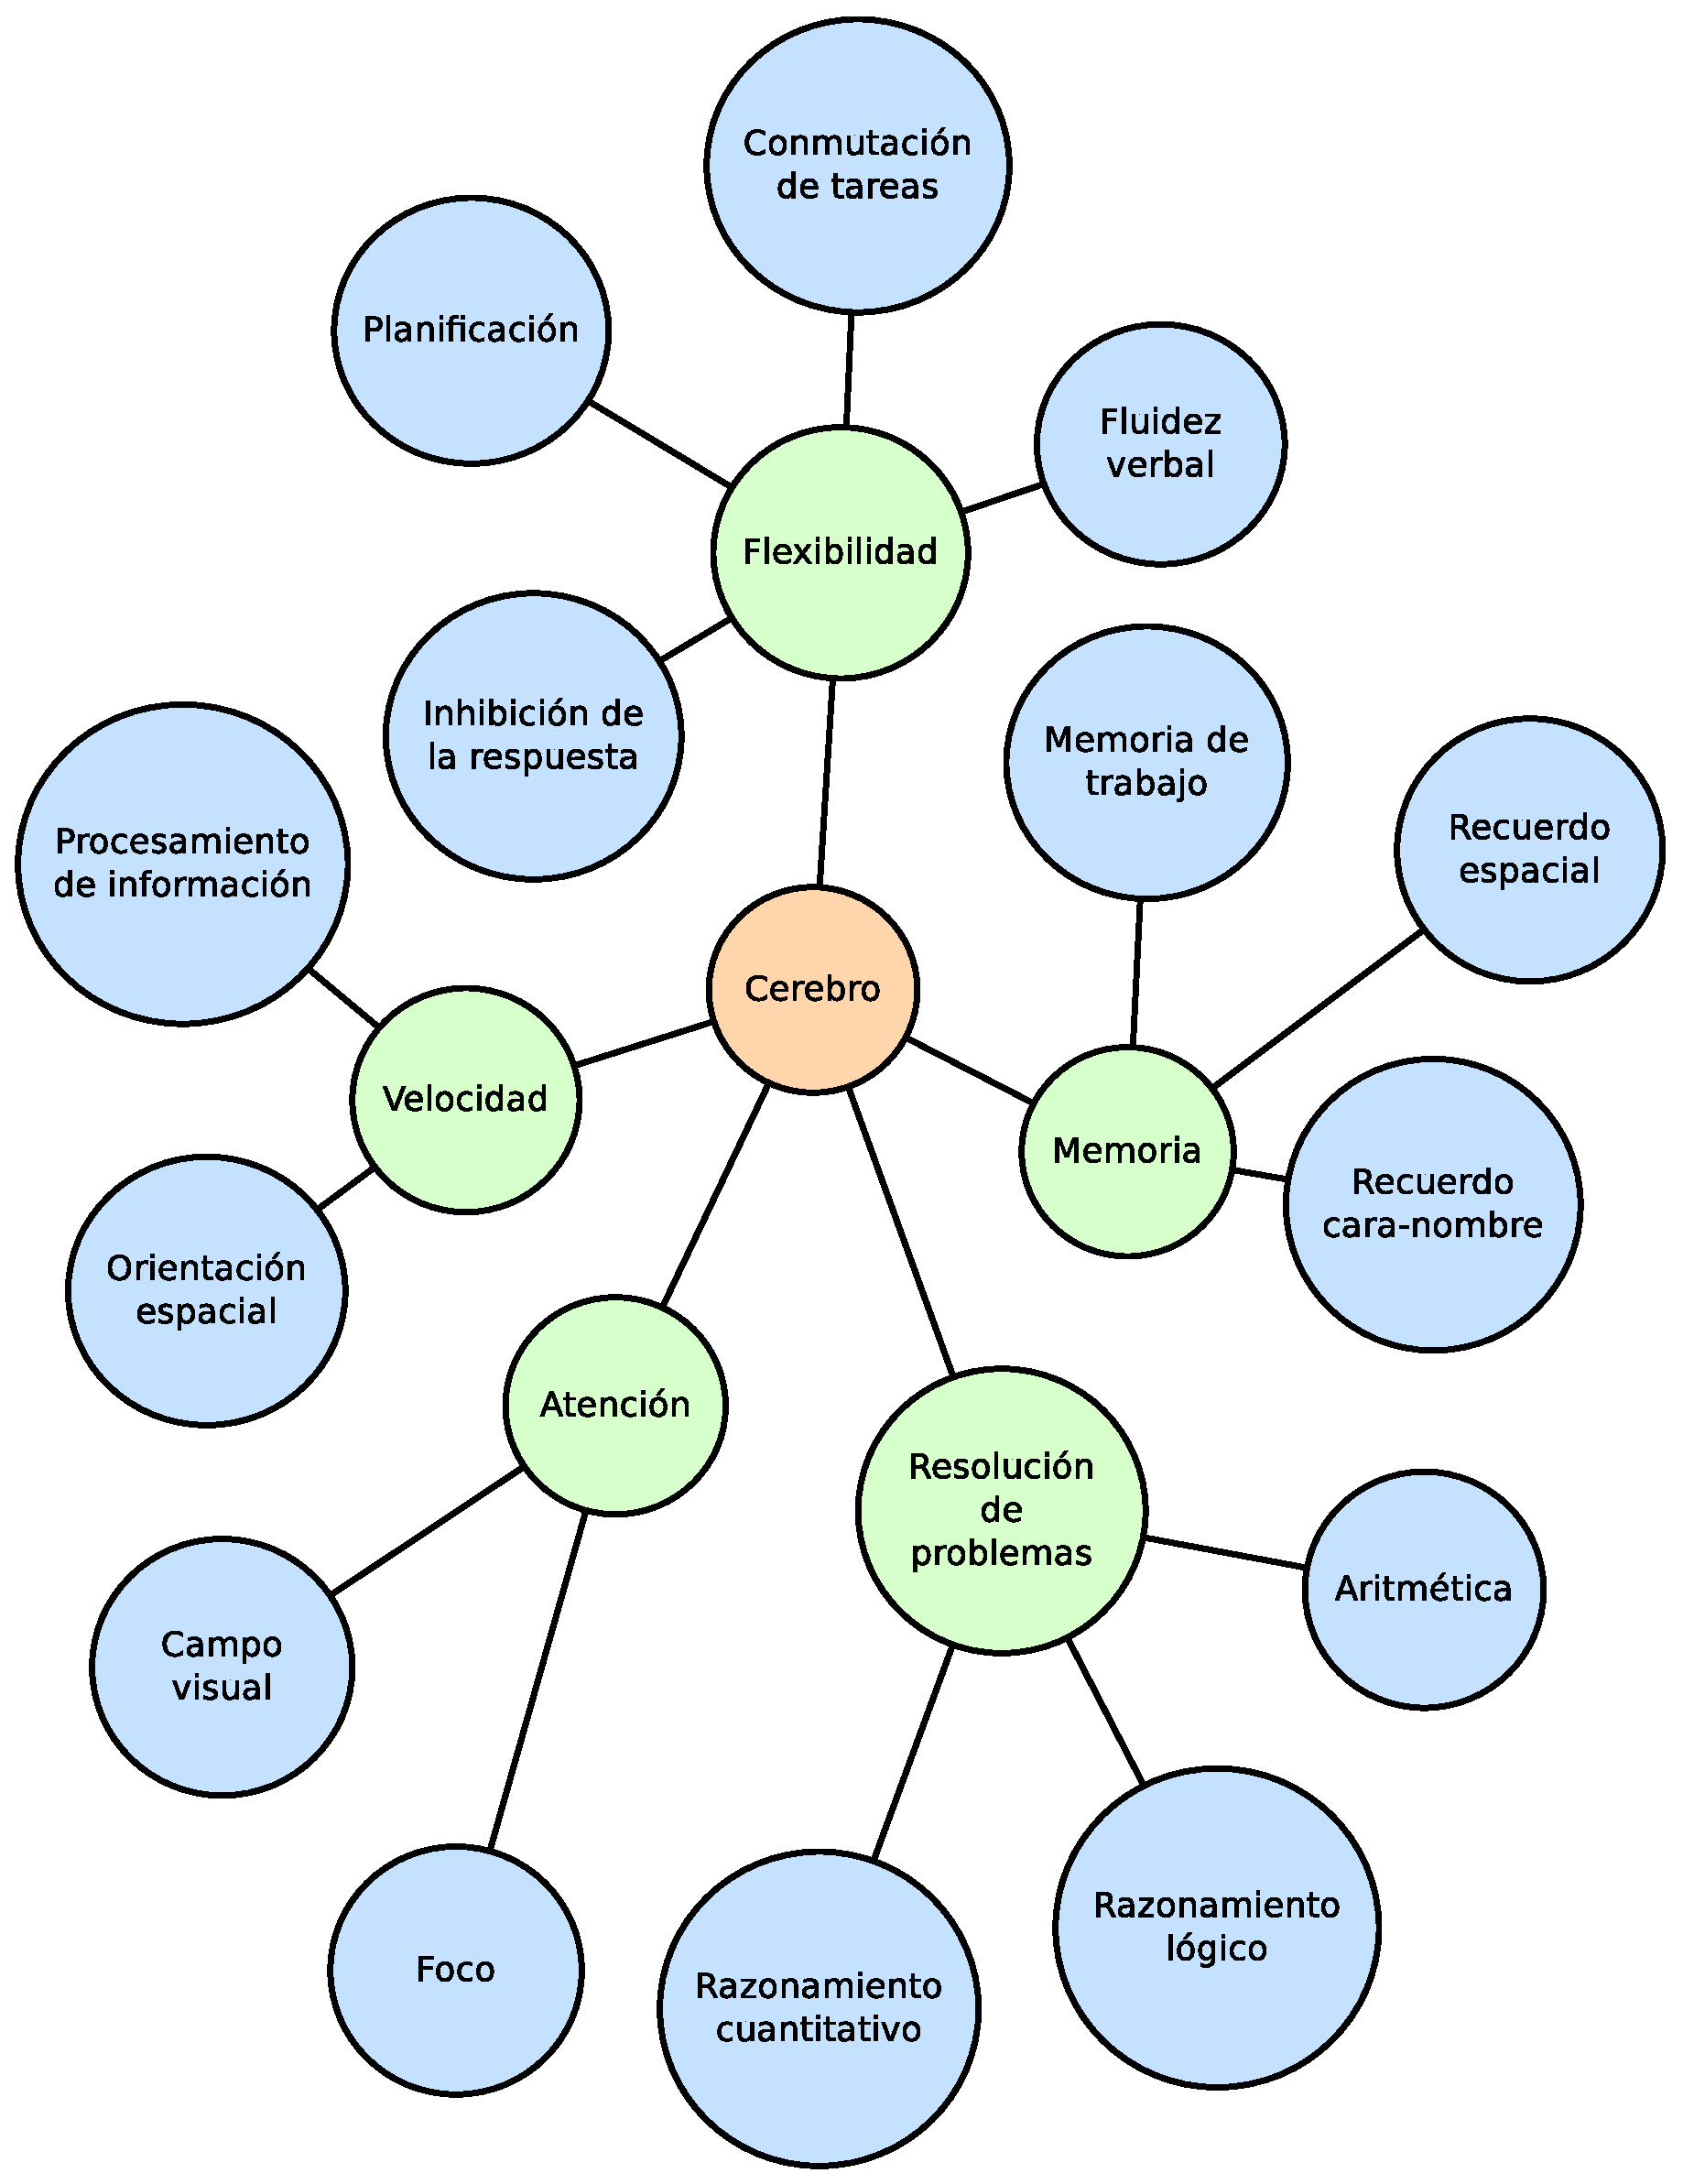
\includegraphics[width=\textwidth]{images/games-diagram-esp.eps}
    \caption{Diagrama de habilidades mentales}
    \label{fig::habilidades}
  \end{center}
\end{figure}

\renewcommand*{\arraystretch}{1.07}
\begin{table}[h]
\begin{small}
\label{table:capacidades}
\begin{center}  
\begin{sideways}
\begin{tabular}{|c|l|l|l|}
\hline
\tabheadformat
\tabhead{Grupo} & \tabhead{Habilidad} & \tabhead{Descripción} & \tabhead{Estimulación} \\
\hline\hline
\multirow{6}{*}{\begin{sideways}Memoria\end{sideways}} & Memoria  & Almacenamiento temporal de información & Mostrar pequeñas cantidades de información para memorizar \\
 & de trabajo & durante el desarrollo de una tarea. & y después requerirlas de algún modo. \\
\cline{2-4}
 & Memoria & Información del entorno, localización de objetos & Ofrecer un paisaje de objetos para su memorización \\
 & espacial & y orientación en el espacio. & y solicitar la reconstrucción del mismo.\\
\cline{2-4}
 & Memoria & Relación entre objetos y etiquetas asociadas & Mostrar la relación existente entre varios objetos y etiquetas.\\
 & nombre-cara & a dichos objetos.& El jugador deberá memorizar esas relaciones y reconstruirlas.\\
\hline

\multirow{6}{*}{\begin{sideways}Res. prob.\end{sideways}} & Aritmética & Realización de operaciones matemáticas & Enfrentar al jugador a gran cantidad de operaciones sencillas\\
 & & sencillas de forma rápida y correcta. & de suma, resta, multiplicación y división.\\
\cline{2-4}
 & Razonamiento & Realización de... & Mostrar... \\
 & lógico & y... & y... \\
\cline{2-4}
 & Razonamiento & Realización de... & Ofrecer... \\
 & cuantitativo & y... & y... \\
\hline

\multirow{4}{*}{\begin{sideways}Atención\end{sideways}} & Concentración & Realización de... & Mostrar... \\
 &  & y... & y... \\
\cline{2-4}
 & Campo & Realización de... & Mostrar... \\
 & visual & y... & y... \\
\hline

\multirow{4}{*}{\begin{sideways}Velocidad\end{sideways}} & Procesamiento & Realización de... &  Ofrecer... \\
 & de Información & y... & y... \\
\cline{2-4}
 & Orientación & Realización de... & Mostrar... \\
 & espacial & y... & y... \\
\hline
\multirow{8}{*}{\begin{sideways}Flexibilidad\end{sideways}} & Control de & Realización de... & Mostrar... \\
 & impulsos & y... & y... \\
\cline{2-4}
& Planificación & Realización de... & Ofrecer... \\
& & y... & y... \\
\cline{2-4}
& Conmutación & Realización de... & Mostrar... \\
& de tareas & y... & y... \\
\cline{2-4}
& Fluidez  & Realización de... & Ofrecer... \\
& verbal  & y... & y... \\
\hline
\end{tabular}
\end{sideways}
\end{center}
\end{small}
\caption{Descripción del entrenamiento de capacidades mentales}
\end{table}


\section{Medición cuantitativa de la evolución cerebral mediante juegos}

A lo largo de esta sección se expondrán los conceptos básicos del diseño de la plataforma, para después desarrollar el sistema de puntuación de partidas y el conjunto de variables cerebrales que posibilitarán, por un lado la medición de la evolución de entrenamiento, y por otro la clasificación y recomendación de usuarios y juegos.

\subsection{Juegos, partidas y actividades puntuables}
\label{sec::juegos-partidas-actividades}

El diseño de BreakBrain hace distinción entre tres conceptos principales: juegos, actividades puntuables y partidas. En la figura \ref{fig::juegos-partidas-actividades} se ofrece una visión gráfica de la relación entre estos términos.

Resulta de vital importancia comprender bien estos conceptos para poder comprender el sistema de medición de la evolución de entrenamiento que ha sido creado en torno a ellos.

\subsubsection{Juego}

Un juego es una pequeña aplicación interactiva, centrada en una única habilidad mental (perteneciente a una capacidad), integrada en la plataforma y que permite su utilización por parte de uno o más usuarios de forma simultánea.

En base a la cantidad de jugadores que puedan enfrentarse entre sí en un juego, distinguimos entre juegos monojugador y juegos multijugador:

\begin{itemize}
\item {\bf Juegos monojugador}

Se trata de juegos diseñados para ser utilizados por un único usuario. No supone ningún tipo de interacción con otros usuarios. En este tipo de juegos no se gana o se pierde, sino que el resultado de los mismos es un valor cuantitativo que indica el grado de éxito de la partida (término que se estudia más adelante).

\item {\bf Juego multijugador}

En este caso se trata de juegos diseñados para ser utilizados por dos jugadores a la vez, suponiendo un enfrentamiento entre ellos. Sólo un jugador de los dos puede ganar cada ronda o partida (término que se estudia más adelante).

\end{itemize}

\subsubsection{Partida}

Una partida es cada una de las instancias jugables de un juego. Para ser más claros, cuando dos jugadores se encuentran jugando al mismo juego individual, cada uno en su máquina y sin realizar interacción alguna con el otro, cada uno de esos jugadores está jugando realmente una partida distinta del mismo juego.

Por otro lado, cuando dos jugadores se enfrentan cara a cara a un juego, compitiendo el uno contra el otro, ambos se encuentran en una misma partida de dicho juego. Obviamente en este caso siempre se tratará de juegos multijugador.

\subsubsection{Actividad puntuable}

La actividad puntuable es la unidad mínima jugable y, por lo tanto, la unidad mínima de entrenamiento y puntuación. Cada partida está compuesta por varias actividades puntuables. Por ejemplo, dado un juego de memoria en el que el usuario tiene que recordar la localización de grupos de objetos, cada actividad puntuable sería cada distribución de objetos a la que el usuario debe enfrentarse y resolver.

En base al número de actividades puntuables que las compongan, distinguimos entre los siguientes tipos de partidas:

\begin{itemize}
\item {\bf Partidas de corta duración}: Partida formada por 10 actividades puntuables
\item {\bf Partidas de duración media}: Partida formada por 30 actividades puntuables
\item {\bf Partidas de larga duración}: Partida formada por 50 actividades puntuables
\end{itemize}

\begin{figure}[H]
  \begin{center}
    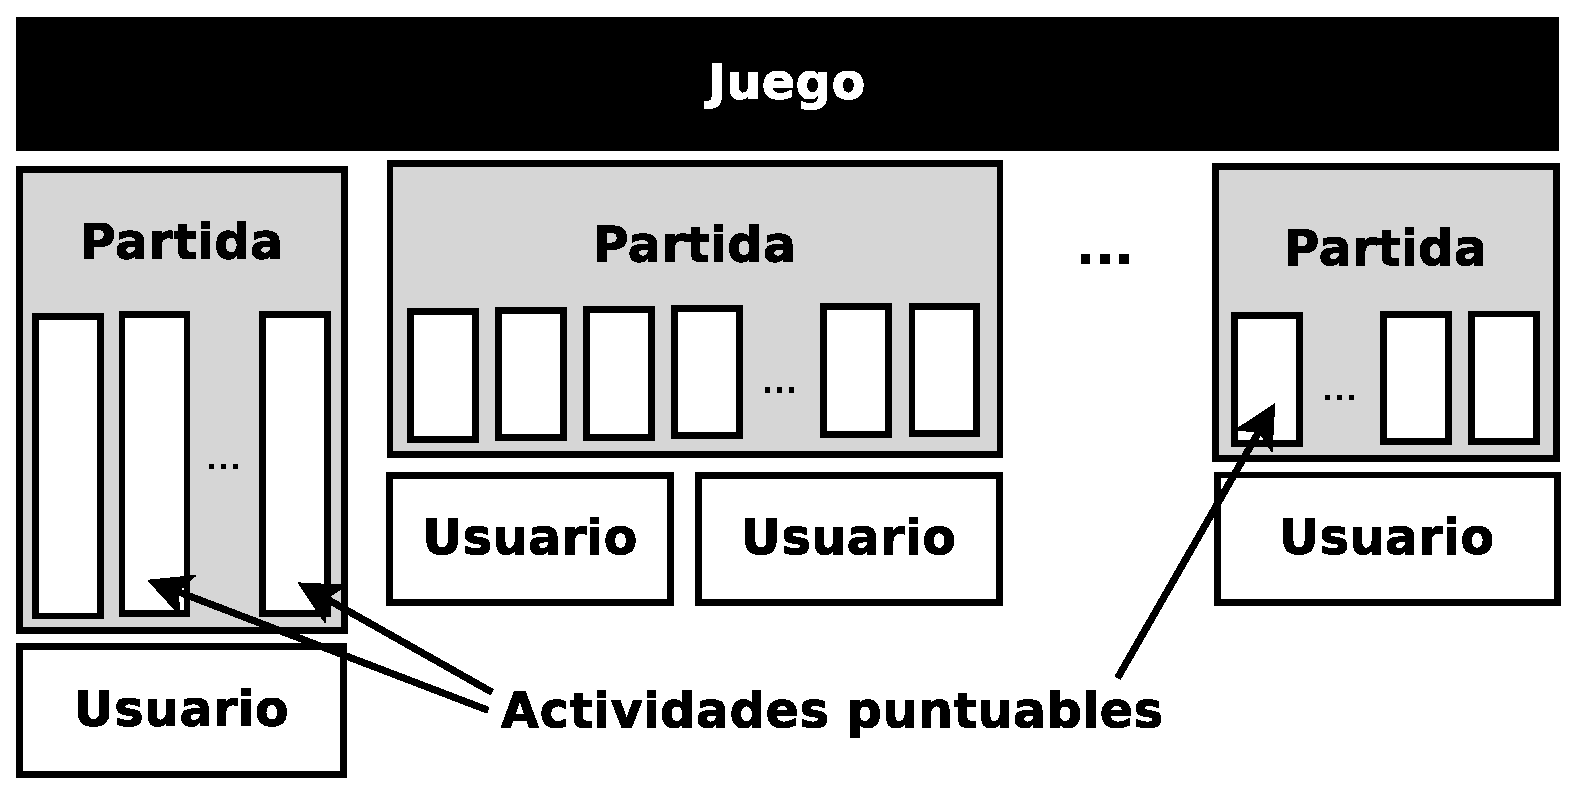
\includegraphics[width=0.8\textwidth]{images/juegos-partidas-actividades.eps}
    \caption{Juegos, partidas y actividades puntuables}
    \label{fig::juegos-partidas-actividades}
  \end{center}
\end{figure}

\subsection{Puntuación de partidas}

Tal y como se ha explicado en la sección \ref{sec::juegos-partidas-actividades}, una partida $p$ está compuesta por varias actividades puntuables $a_i$. La puntuación de una partida, $s_{p}$, es la suma de las puntuaciones obtenidas en cada actividad puntuable:


\begin{equation}
s_{p} = \sum\limits_{i = 0}^A s_i
\label{eq:partida}
\end{equation}

siendo $A$ el número total de actividades puntuables completadas en la partida $p$, y $s_i$ la puntuación de cada una de esas actividades.

La puntuación de cada actividad, $s_i$, se basa en dos aspectos: el tiempo empleado para completarla, $t_i$, y la valoración de éxito de la misma, $e_i$. Esta valoración de éxito puede ser satisfactoria o no satisfactoria, lo que matemáticamente se traduce en un 1 o un 0. Por otro lado, el tiempo $t_i$ debe encontrarse normalizado entre 0 y 1, para lo cual basta con dividir el tiempo empleado en realizar la actividad $i$ entre el tiempo empleado en realizar la actividad que más duración haya tenido. Teniendo en cuenta ambos aspectos, la puntuación de una actividad puntuable $a_i$ es la siguiente:

\begin{equation}
s_i = \frac{1}{t_i} \cdot e_i
\end{equation}

Reemplazando esta expresión en la ecuación \ref{eq:partida}, tenemos:

\begin{equation}
s_{p} = \sum\limits_{i = 0}^A \frac{1}{t_i} \cdot e_i
\end{equation}

Las actividades puntuables que no hayan sido completadas reciben una puntuación $s_i = 0$. Dependiendo del tipo de partida, será o no posible darla por finalizada sin haber completado todas las actividades puntuables que la constituyen:

\begin{itemize}
\item {\bf Puntuación en partidas monojugador}: el jugador recibe los puntos obtenidos en todas las actividades puntuables que constituyen la partida al finalizar la misma.
\item {\bf Puntuación en partidas multijugador}: una vez finalizadas todas las actividades puntuables de la partida por parte de uno de los jugadores, éste es considerado vencedor y la partida termina. Ambos jugadores reciben los puntos obtenidos durante la misma. En el caso del jugador perdedor, recibirá la puntuación de las actividades puntuables que haya completado satisfactoriamente antes de que el otro jugador haya terminado.
\end{itemize}

Teniendo en cuenta todo lo anterior, una partida $p$ formada por $A$ actividades puntuables tendrá una puntuación $s_p$ tal que $0 \leq s_p \leq A$.

\subsection{Variables de clasificación}

El perfil de cada usuario contiene la puntuación de cada habilidad cerebral, calculada mediante la suma de las puntuaciones obtenidas en cada partida de cada juego destinado a estimular esa habilidad. Además de ello contiene otras variables, como la cantidad de partidas ganadas, el sexo del individuo, etc. Todas estas variables se clasifican en 3 grupos:

\subsubsection{Variables estáticas o de agrupación}

\begin{itemize}
\item {\tt sex}: Sexo (hombre o mujer)
\item {\tt age}: Edad
\item {\tt keywords}: Palabras clave
\item {\tt training-interests}: Lista de habilidades mentales que el usuario está interesado en entrenar
\end{itemize}

\subsubsection{Variables dinámicas mentales}

\begin{itemize}
\item {\tt memory}: puntuación en el área de Memoria. Se trata de la suma de las siguientes tres puntuaciones:
  \begin{itemize}
  \item {\tt working-memory}: puntuación en memoria de trabajo.
  \item {\tt spatial-memory}: puntuación en memoria espacial
  \item {\tt face-name}: puntuación en memoria de asociación nombre-cara
  \end{itemize}
\item {\tt problem-solving}: puntuación en el área de Resolución de problemas. Se calcula mediante la suma de las siguientes tres puntuaciones:
  \begin{itemize}
  \item {\tt arithmetic}: puntuación en aritmética.
  \item {\tt logical-reasoning}: puntuación en razonamiento lógico.
  \item {\tt quantitative-reasoning}: puntuación en razonamiento cuantitativo.
  \end{itemize}
\item {\tt attention}: puntuación en la capacidad de Atención. Su valor es la suma de los valores de las siguientes dos variables:
  \begin{itemize}
  \item {\tt focus}: puntuación en la habilidad de concentración
  \item {\tt visual-field}: puntuación en campo visual
  \end{itemize}
\item {\tt speed}: puntuación en el área de Velocidad de procesamiento. Se trata de la suma de las siguientes dos variables:
  \begin{itemize}
  \item {\tt information-processing}: puntuación en procesamiento de la información
  \item {\tt spatial-orientation}: puntuación en orientación espacial
  \end{itemize}
\item {\tt flexibility}: puntuación en la capacidad de Flexibilidad. Se computa mediante la suma de las siguientes cuatro variables:
  \begin{itemize}
  \item {\tt response-inhibition}: puntuación en control de impulsos
  \item {\tt planning}: puntuación en planificación
  \item {\tt task-switching}: puntuación en conmutación de tareas
  \item {\tt verbal-fluency}: puntuación en fluidez verbal
  \end{itemize}
\end{itemize}

\subsubsection{Variables dinámicas sociales}

\begin{itemize}
\item {\tt followers}: cantidad de personas que siguen al usuario.
\item {\tt followees}: cantidad de personas a las que el usuario sigue.
\end{itemize}



% <<<<<<<<<<<<<<<<<<<<<<<<<<<<<<

\section{Sistema de recomendación}


\subsection{Algoritmo de recomendación de usuarios}

\subsection{Algoritmo de recomendación de juegos}

\subsection{Notas personales}

En \ref{sec::estructuras-primarias} se habla de la generación de patrones. Esto hay que comentarlo en los juegos.

En \ref{sec::corteza-cerebral} se habla de las áreas de Brodmann. Debería tenerlas en cuenta ne los juegos. La experiencia en la determinación de las representaciones corticales.

En \ref{sec::estructuras-subcorticales} se habla de como la experiencia afecta al cerebro

%\section{Algoritmo de búsqueda de usuarios}
